\documentclass{beamer}

\pdfmapfile{+sansmathaccent.map}


\mode<presentation>
{
	\usetheme{Warsaw} % or try Darmstadt, Madrid, Warsaw, Rochester, CambridgeUS, ...
	\usecolortheme{seahorse} % or try seahorse, beaver, crane, wolverine, ...
	\usefonttheme{serif}  % or try serif, structurebold, ...
	\setbeamertemplate{navigation symbols}{}
	\setbeamertemplate{caption}[numbered]
} 


%%%%%%%%%%%%%%%%%%%%%%%%%%%%
% itemize settings

\definecolor{mypaleblue}{RGB}{240, 240, 255}
\definecolor{mylightblue}{RGB}{120, 150, 255}
\definecolor{myblue}{RGB}{90, 90, 255}
\definecolor{mygblue}{RGB}{70, 110, 240}
\definecolor{mydarkblue}{RGB}{0, 0, 180}
\definecolor{myblackblue}{RGB}{40, 40, 120}

\definecolor{mygreen}{RGB}{0, 200, 0}
\definecolor{mydarkgreen}{RGB}{0, 120, 0}
\definecolor{mygreen2}{RGB}{245, 255, 230}

\definecolor{mygray}{gray}{0.8}
\definecolor{mygray2}{RGB}{130, 130, 130}
\definecolor{mydarkgray}{RGB}{80, 80, 160}
\definecolor{mylightgray}{RGB}{160, 160, 160}

\definecolor{mydarkred}{RGB}{160, 30, 30}
\definecolor{mylightred}{RGB}{255, 150, 150}
\definecolor{myred}{RGB}{200, 110, 110}
\definecolor{myblackred}{RGB}{120, 40, 40}

\definecolor{mypink}{RGB}{255, 30, 80}
\definecolor{myhotpink}{RGB}{255, 80, 200}
\definecolor{mywarmpink}{RGB}{255, 60, 160}
\definecolor{mylightpink}{RGB}{255, 80, 200}
\definecolor{mydarkpink}{RGB}{155, 25, 60}

\definecolor{mydarkcolor}{RGB}{60, 25, 155}
\definecolor{mylightcolor}{RGB}{130, 180, 250}

\setbeamertemplate{itemize items}[default]

\setbeamertemplate{itemize item}{\color{myblackblue}$\blacksquare$}
\setbeamertemplate{itemize subitem}{\color{mydarkblue}$\blacktriangleright$}
\setbeamertemplate{itemize subsubitem}{\color{mygray}$\blacksquare$}

\setbeamercolor{palette quaternary}{fg=white,bg=mygblue} %mydarkgray
\setbeamercolor{titlelike}{parent=palette quaternary}

\setbeamercolor{palette quaternary2}{fg=white,bg=mygblue}%black myblue
\setbeamercolor{frametitle}{parent=palette quaternary2}

\setbeamerfont{frametitle}{size=\Large,series=\scshape}
\setbeamerfont{framesubtitle}{size=\normalsize,series=\upshape}


%%%%%%%%%%%%%%%%%%%%%%%%%%%%
% block settings

%\setbeamercolor{block title}{bg=red!50,fg=black}
%\setbeamercolor{block title}{bg=mylightblue,fg=black}
\setbeamercolor{block title}{bg=myblackblue,fg=white}

\setbeamercolor*{block title example}{bg=mygreen!40!white,fg=black}

\setbeamercolor*{block body example}{fg= black,
	bg= mygreen2}


%%%%%%%%%%%%%%%%%%%%%%%%%%%%
% URL settings
\hypersetup{
	colorlinks=false,
	linkcolor=blue,
	filecolor=blue,      
	urlcolor=blue,
}

%%%%%%%%%%%%%%%%%%%%%%%%%%

\renewcommand{\familydefault}{\rmdefault}

\usepackage{amsmath}
\usepackage{mathtools}

\usepackage{subcaption}

\usepackage{qrcode}

\newcommand{\bo}[1] {\mathbf{#1}}
\newcommand{\R}{\mathbb{R}} 
\newcommand{\T}{^\top}     



\newcommand{\mydate}{Spring 2025}

\newcommand{\mygit}{\textcolor{blue}{\href{https://github.com/SergeiSa/Computational-Intelligence-2025}{github.com/SergeiSa/Computational-Intelligence-2025}}}

\newcommand{\myqr}{ \textcolor{black}{\qrcode[height=1.5in]{https://github.com/SergeiSa/Computational-Intelligence-2025}}
}

\newcommand{\myqrframe}{
	\begin{frame}
		\centerline{Lecture slides are available via Github, links are on Moodle:}
		\bigskip
		\centerline{\mygit}
		\bigskip
		\myqr
	\end{frame}
}


\newcommand{\bref}[2] {\textcolor{blue}{\href{#1}{#2}}}



%%%%%%%%%%%%%%%%%%%%%%%%%%%%
% code settings

\usepackage{listings}
\usepackage{color}
% \definecolor{mygreen}{rgb}{0,0.6,0}
% \definecolor{mygray}{rgb}{0.5,0.5,0.5}
\definecolor{mymauve}{rgb}{0.58,0,0.82}
\lstset{ 
	backgroundcolor=\color{white},   % choose the background color; you must add \usepackage{color} or \usepackage{xcolor}; should come as last argument
	basicstyle=\footnotesize,        % the size of the fonts that are used for the code
	breakatwhitespace=false,         % sets if automatic breaks should only happen at whitespace
	breaklines=true,                 % sets automatic line breaking
	captionpos=b,                    % sets the caption-position to bottom
	commentstyle=\color{mygreen},    % comment style
	deletekeywords={...},            % if you want to delete keywords from the given language
	escapeinside={\%*}{*)},          % if you want to add LaTeX within your code
	extendedchars=true,              % lets you use non-ASCII characters; for 8-bits encodings only, does not work with UTF-8
	firstnumber=0000,                % start line enumeration with line 0000
	frame=single,	                   % adds a frame around the code
	keepspaces=true,                 % keeps spaces in text, useful for keeping indentation of code (possibly needs columns=flexible)
	keywordstyle=\color{blue},       % keyword style
	language=Octave,                 % the language of the code
	morekeywords={*,...},            % if you want to add more keywords to the set
	numbers=left,                    % where to put the line-numbers; possible values are (none, left, right)
	numbersep=5pt,                   % how far the line-numbers are from the code
	numberstyle=\tiny\color{mygray}, % the style that is used for the line-numbers
	rulecolor=\color{black},         % if not set, the frame-color may be changed on line-breaks within not-black text (e.g. comments (green here))
	showspaces=false,                % show spaces everywhere adding particular underscores; it overrides 'showstringspaces'
	showstringspaces=false,          % underline spaces within strings only
	showtabs=false,                  % show tabs within strings adding particular underscores
	stepnumber=2,                    % the step between two line-numbers. If it's 1, each line will be numbered
	stringstyle=\color{mymauve},     % string literal style
	tabsize=2,	                   % sets default tabsize to 2 spaces
	title=\lstname                   % show the filename of files included with \lstinputlisting; also try caption instead of title
}

%%%%%%%%%%%%%%%%%%%%%%%%%%%%
% tikz settings

\usepackage{tikz}
\tikzset{every picture/.style={line width=0.75pt}}

%%%%%%%%%%%%%%%%%%%%%%%%%%%%




\title{Optimization problems, Analytic solutions}
\subtitle{Computational Intelligence, Lecture 4}
\author{by Sergei Savin}
\centering
\date{\mydate}



\begin{document}
\maketitle


\begin{frame}{Content}

\begin{itemize}
\item Optimization problem
\item Feasibility problem
\item Norms and quadratic forms
\item Problems with analytical solutions
\item Weighted pseudoinverse
\end{itemize}

\end{frame}




\begin{frame}{Optimization problem}
	% \framesubtitle{Parameter estimation}
	\begin{flushleft}
		
		An optimization problem has the following form:
		%
		\begin{equation}
			\begin{aligned}
				& \underset{\text{decision variables}}{\text{minimize}}
				& & \text{cost function}, \\
				& \text{subject to}
				& & \text{constraints}.
			\end{aligned}
		\end{equation}
	
		Where the solution to the optimization problem is the optimal value of the decision variables.
		
		\bigskip
		
		For example:
		%
		\begin{equation}
			\begin{aligned}
				& \underset{\bo{x}}{\text{minimize}}
				& & f(\bo{x}), \\
				& \text{subject to}
				& & \begin{cases}
					g(\bo{x}) = 0, \\
					h(\bo{x}) \leq 0.
				\end{cases}
			\end{aligned}
		\end{equation}
	
	In this example, $\bo{x} \in \R^n$ is the decision variable, $f(\bo{x}): \ \R^n \rightarrow \R$ is a cost function, $g(\bo{x}) = 0$ are equality constraints, and $h(\bo{x}) \leq 0$ are inequality constraints.

	\end{flushleft}
\end{frame}



\begin{frame}{Feasibility problem}
	% \framesubtitle{Parameter estimation}
	\begin{flushleft}
		
		A cost function is always scalar. A special case of a cost function is a constant:
		%
		\begin{equation}
			\begin{aligned}
				& \underset{\bo{x}}{\text{minimize}}
				& & 0, \\
				& \text{subject to}
				& & \begin{cases}
					g(\bo{x}) = 0, \\
					h(\bo{x}) \leq 0.
				\end{cases}
			\end{aligned}
		\end{equation}
	
		In this case any $\bo{x}$ that satisfies constraints would be a solution to the problem. It is called a \emph{feasibility problem}. We solved this type of problems to find out if there exist any $\bo{x}$ that satisfies constraints.
		
	\end{flushleft}
\end{frame}




\begin{frame}{Unconstrained optimization}
	% \framesubtitle{Parameter estimation}
	\begin{flushleft}
		
		Often an optimization problem would not feature constraints:
		%
		\begin{equation}
			\begin{aligned}
				& \underset{\bo{x}}{\text{minimize}}
				& & f(\bo{x})
			\end{aligned}
		\end{equation}
		
		We can call it \emph{unconstrained optimization}.
		
		\bigskip
		
		Note that the decision variable $\bo{x}$ can belong to a set $\bo{x} \in \mathcal{X}$ or the cost function may have a domain $f: \ \mathcal{D} \rightarrow \R$; in these cases, the set of allowed values of $\bo{x}$, as well as the domain of the function represent \emph{implicit} constraints. 
		
		\bigskip
		
		For example, the problem:
		
		$$\underset{x}{\text{minimize}} \ \ \ln x$$
		
		has an implicit constraint $x \geq 0$.
		
	\end{flushleft}
\end{frame}



\begin{frame}{Equatily constraints, Lagrangian}
	% \framesubtitle{Parameter estimation}
	\begin{flushleft}
		
		Consider optimization problems with equality constraints:
		%
		\begin{equation}
			\begin{aligned}
				& \underset{\bo{x}}{\text{minimize}}
				& & f(\bo{x}), \\
				& \text{subject to}
				& & g(\bo{x}) = 0
			\end{aligned}
		\end{equation}
		
		We solve it by constructing its \emph{Lagrangian}:
		
		\begin{equation}
			L(\bo{x}, \lambda) = f(\bo{x}) + \lambda\T g(\bo{x})
		\end{equation}
		
		Extremum of the Lagrangian corresponds to the solution of the original problem:
		
		\begin{align}
			\frac{\partial L(\bo{x}, \lambda)}{\partial \bo{x}} = 0
			\\
			\frac{\partial L(\bo{x}, \lambda)}{\partial \lambda} = 0
		\end{align}
		
	\end{flushleft}
\end{frame}



\begin{frame}{Unconstrained optimization examples}
% \framesubtitle{Parameter estimation}
\begin{flushleft}
	

Some types of optimization problems admit an analytic solution. For example:
	

Problem 1. $\text{minimize} \ ||\mathbf{x}||$. \textcolor{white}{Solution $\mathbf{x} = \mathbf{0}$} 

\bigskip

Problem 2. $\text{minimize} \ ||\mathbf{A}\mathbf{x}||$. \textcolor{white}{Solution $\mathbf{x} = \mathbf{0}$.}

\bigskip

Problem 3. $\text{minimize} \ ||\mathbf{A}\mathbf{x} + \mathbf{b}||$. 

\bigskip

We know solution of $\textcolor{mydarkgray}{\text{minimize} \ ||\mathbf{A}\mathbf{x} - \mathbf{b}||}$, which is $\mathbf{x} = \mathbf{A}^+ \mathbf{b}$. Therefore the problem 3 has a solution $\mathbf{x} = -\mathbf{A}^+ \mathbf{b}$.
 
\end{flushleft}
\end{frame}



\begin{frame}{Least squares with constraints}
\begin{flushleft}


Problem 4. (form 1)
%
\begin{equation}
\begin{aligned}
& \underset{\mathbf{x}}{\text{minimize}}
& & || \mathbf{x} ||, \\
& \text{subject to}
& & \mathbf{A} \mathbf{x} = \mathbf{b}.
\end{aligned}
\end{equation}


All solutions to $\mathbf{A} \mathbf{x} = \mathbf{b}$ are written as $\mathbf{x} = \mathbf{A}^+\mathbf{b} + \mathbf{N}\mathbf{z}$, where $\mathbf{N} = \text{null}(\mathbf{A})$, and $\mathbf{A}^+\mathbf{b} \in \text{row}(\mathbf{A})$ as we proved previously. 

\bigskip

Since the null space solution $\mathbf{N}\mathbf{z}$ and the row space paricular solution $\mathbf{A}^+\mathbf{b}$ are orthogonal, the minimum norm solution corresponds to $\mathbf{z} = \mathbf{0}$, hence:

\begin{equation}
	\mathbf{x} = \mathbf{A}^+\mathbf{b}
\end{equation}

\end{flushleft}
\end{frame}

\begin{frame}{Least squares with constraints}
\begin{flushleft}


Thus, the solution is  $\mathbf{x} = \mathbf{A}^+\mathbf{b}$. Notice that the solutions for the problems 3 and 4 are written identically (sans the sign), even though the problem 3 asks to minimize the residual of the linear system, while problem 4 - to find the minimum-norm solution. 

\bigskip

This illustrates an important fact: the solution to the least squares problem, formulated either as ``minimization of a residual" or as a ``minimum norm solution" are given by the same formula, which we call Moore-Penrose pseudoinverse.


\end{flushleft}
\end{frame}




\begin{frame}{Least squares with constraints}
	\begin{flushleft}
		
		
		Problem 4. (form 2)
		%
		\begin{equation}
			\begin{aligned}
				& \underset{\mathbf{x}}{\text{minimize}}
				& & \frac{1}{2} \bo{x}\T \bo{x}, \\
				& \text{subject to}
				& & \bo{A} \bo{x} = \bo{b}.
			\end{aligned}
		\end{equation}
		
		Let us find Lagrangian $L =\frac{1}{2} \bo{x}\T \bo{x} + \lambda\T ( \mathbf{A} \mathbf{x} - \bo{b})$. It achieves extremum at solution of the original problem:
		
		\begin{align}
			\frac{\partial L}{\partial \bo{x}} &=  \bo{x} + \bo{A}\T  \lambda = 0 
			\\
			\frac{\partial L}{\partial \lambda} &=  \bo{A} \bo{x}- \bo{b} = 0
		\end{align}
		
		We can express $\bo{x} = -\bo{A}\T  \lambda$ and substitute it $\bo{A} \bo{A}\T  \lambda= -\bo{b}$. If $\text{det}(\bo{A} \bo{A}\T ) \neq 0$, then:
		%
		\begin{align}
			 \lambda= - (\bo{A} \bo{A}\T )^{-1} \bo{b}
			 \\
			 \bo{x} = \bo{A}\T  (\bo{A} \bo{A}\T )^{-1} \bo{b}
		\end{align}		
		
	\end{flushleft}
\end{frame}




\begin{frame}{Least squares with constraints}
	\begin{flushleft}
		
		We can prove that $ \bo{A}\T  (\bo{A} \bo{A}\T )^{-1} = \bo{A}^+$.
		
		\bigskip
		
		We can re-write the expression $\bo{A} \bo{A}\T  \lambda= -\bo{b}$ using SVD decomposition $\bo{A} = \bo{C}\Sigma\bo{R}\T$:
		
		\begin{align}
			 \bo{C}\Sigma\bo{R}\T \bo{R}\Sigma\bo{C}\T  \lambda= -\bo{b}
			 \\
			 \bo{C}\Sigma \Sigma\bo{C}\T  \lambda= -\bo{b}
			 \\
			  \textcolor{mydarkred}{\bo{C}\T  \lambda}= -\Sigma^{-2} \bo{C}\T \bo{b}
		\end{align}				
		
		Next, we do the same with $\bo{x} = -\bo{A}\T  \lambda$:
		%
		\begin{align}
			\bo{x} = -\bo{R}\Sigma\textcolor{mydarkred}{\bo{C}\T  \lambda}
			\\
			\bo{x} = \bo{R}\Sigma\Sigma^{-2} \bo{C}\T \bo{b}
			\\
			\bo{x} = \bo{R}\Sigma^{-1} \bo{C}\T \bo{b}
		\end{align}				
		
		But $ \bo{R}\Sigma^{-1} \bo{C}\T \ = \bo{A}^+$, so $\bo{x} =\bo{A}^+ \bo{b}$. More in Appendix.
		
	\end{flushleft}
\end{frame}







\begin{frame}{Problems with weighted norms}
%\framesubtitle{Part 4}
\begin{flushleft}

Problem 5. 
%
\begin{equation}
\begin{aligned}
& \underset{\mathbf{x}}{\text{minimize}}
& & || \mathbf{D}\mathbf{x} ||, \\
& \text{subject to}
& & \mathbf{A} \mathbf{x} = \mathbf{b}.
\end{aligned}
\end{equation}

One way to think about it is to first find all solution to the constraint equation $\mathbf{A} \mathbf{x} = \mathbf{b}$ and then find optimal one among them. As we know, all solutions are given as: $\mathbf{x} = \mathbf{A}^+\mathbf{b} + \mathbf{N}\mathbf{z}$, where $\mathbf{N} = \text{null}(\mathbf{A})$. Then our cost function becomes: $|| \mathbf{D}\mathbf{A}^+\mathbf{b} +  \mathbf{D}\mathbf{N}\mathbf{z} ||$, which is equivalent to the problem 3. Thus, we can write solution as: 
$\mathbf{z}^* = -(\mathbf{D}\mathbf{N})^+ \mathbf{D}\mathbf{A}^+\mathbf{b}$. In terms of $\mathbf{x}$ solution is:

\begin{equation}
    \mathbf{x}^* = \mathbf{A}^+\mathbf{b}-\mathbf{N}(\mathbf{D}\mathbf{N})^+ \mathbf{D}\mathbf{A}^+\mathbf{b}
\end{equation}
\begin{equation}
	\mathbf{x}^* =( \mathbf{I}-\mathbf{N}(\mathbf{D}\mathbf{N})^+ \mathbf{D})\mathbf{A}^+\mathbf{b}
\end{equation}

\end{flushleft}
\end{frame}



\begin{frame}{Problems with weighted norms}
%\framesubtitle{Part 5}
\begin{flushleft}

Problem 6. 
%
\begin{equation}
\begin{aligned}
& \underset{\mathbf{x}}{\text{minimize}}
& & || \mathbf{D}\mathbf{x} + \mathbf{f} ||, \\
& \text{subject to}
& & \mathbf{A} \mathbf{x} = \mathbf{b}.
\end{aligned}
\end{equation}

After the same initial step, we arrive at the cost function $|| \mathbf{D}\mathbf{N}\mathbf{z} + \mathbf{D}\mathbf{A}^+\mathbf{b} + \mathbf{f}||$. It is only different in the constant term, and the solution is found as follows:


\begin{equation}
    \mathbf{z}^* = -(\mathbf{D}\mathbf{N})^+ (\mathbf{D}\mathbf{A}^+\mathbf{b} + \mathbf{f})
\end{equation}
\begin{equation}
    \mathbf{x}^* = \mathbf{A}^+\mathbf{b}-\mathbf{N}(\mathbf{D}\mathbf{N})^+ (\mathbf{D}\mathbf{A}^+\mathbf{b} + \mathbf{f})
\end{equation}


\end{flushleft}
\end{frame}




\begin{frame}{Positive-definite matrices}
	\begin{flushleft}
		
		A symmetric positive-definite matrix $\bo{M}$ has the following properties:
		
		\begin{align}
			&\bo{M} = \bo{M}\T
			\\
			&\bo{x}\T \bo{M} \bo{x} > 0, \ \ \forall \bo{x} \neq 0
			\\
			& \text{det}(\bo{M}) \neq 0
		\end{align}
		
		Positive-definite matrices (with non-repeating eigenvalues) have orthogonal eigenvectors, making their eigenbasis orthonormal:
		
		\begin{align}
			& \bo{M} \bo{V} = \bo{V} \Lambda  
			\\
			& \bo{M} = \bo{V} \Lambda \bo{V}\T 
		\end{align}
		
	\end{flushleft}
\end{frame}




\begin{frame}{Matrix square root}
	\begin{flushleft}
		
		For a symmetric positive-definite matrix $\bo{M}$ we can define a square root:
		
		\begin{align}
			\bo{M} &= \sqrt{\bo{M} } \sqrt{\bo{M} }
			\\
			\bo{M} &= \bo{M}^\frac{1}{2} \bo{M}^\frac{1}{2}
		\end{align}
		
		We can find a square root via eigendecomposition:
		
		\begin{align}
			& \bo{M} = \bo{V} \Lambda \bo{V}\T 
			\\
			&  \Lambda =  \bo{F} \bo{F}
			\\
			& \bo{M} = \bo{V} \bo{F} \bo{F} \bo{V}\T 
			\\
			& \bo{M} = \bo{V} \bo{F} \bo{V}\T\bo{V}  \bo{F} \bo{V}\T 
			\\
			& \sqrt{\bo{M} }  = \bo{V} \bo{F} \bo{V}\T
			\\
			&\bo{M} = \sqrt{\bo{M} } \sqrt{\bo{M} } 
		\end{align}
		
		
		
	\end{flushleft}
\end{frame}




\begin{frame}{Problems quadratic cost}
\begin{flushleft}

Problem 7. 
%
\begin{equation}
\begin{aligned}
& \underset{\mathbf{x}}{\text{minimize}}
& & \mathbf{x}^\top \mathbf{H} \mathbf{x} + \mathbf{c}^\top\mathbf{x}, \\
& \text{subject to}
& & \mathbf{A} \mathbf{x} = \mathbf{b}.
\end{aligned}
\end{equation}

where $\mathbf{H}$ is positive-definite.

\bigskip

Assume that we found a decomposition $\mathbf{H} = \mathbf{D}^\top\mathbf{D}$. We can also find such $\mathbf{f}$ that $2\mathbf{f}^\top\mathbf{D} = \mathbf{c}^\top$. Then our cost function becomes $\mathbf{x}^\top \mathbf{D}^\top\mathbf{D} \mathbf{x} + 2\mathbf{f}^\top\mathbf{D}\mathbf{x}$, which as we saw before has coinciding minimum with the cost function $||\mathbf{D}\mathbf{x} + \mathbf{f}||$.

\bigskip

Therefore the problem has the same solution as Problem 5, after the mentioned above change in constants.

\end{flushleft}
\end{frame}



\begin{frame}{Weighted pseudoinverse, unconstrained type}
	% \framesubtitle{Parameter estimation}
	\begin{flushleft}
		
		Consider a weighted pseudoinverse problem:
		%
		\begin{align}
			\text{minimize} \ \ ||\bo{A}\bo{x}-\bo{b}||_\bo{W}
		\end{align}		
		%
		where $||\bo{x}||_\bo{W} = \sqrt{\bo{x}\T\bo{W}\bo{x}}$ and $\bo{W} > 0$. We can re-write the problem as:
		%
		\begin{align}
			\text{minimize} \ \ (\bo{A}\bo{x}-\bo{b})\T\bo{W}^\frac{1}{2}\bo{W}^\frac{1}{2}(\bo{A}\bo{x}-\bo{b})
		\end{align}
		
		But this is the same as solving least-squares problem for equality $\bo{W}^\frac{1}{2}\bo{A}\bo{x}=\bo{W}^\frac{1}{2}\bo{b}$, which is does via Moore-Penrose pseudoinverse:
		%
		\begin{align}
			\bo{x}=(\bo{W}^\frac{1}{2}\bo{A})^+\bo{W}^\frac{1}{2}\bo{b}
		\end{align}
		
	\end{flushleft}
\end{frame}


\begin{frame}{Weighted pseudoinverse, constrained type}
	% \framesubtitle{Parameter estimation}
	\begin{flushleft}
		
		Consider a weighted pseudoinverse problem:
		%
		\begin{equation}
			\begin{aligned}
				& \underset{\bo{x}}{\text{minimize}}
				& & \bo{x}\T \bo{W} \bo{x}, \\
				& \text{subject to}
				& & \bo{A}\bo{x}=\bo{b}
			\end{aligned}
		\end{equation}
		
		We can use Lagrange multipliers to rewrite the problem as minimization of the function $L(\bo{x}, \lambda) = \bo{x}\T \bo{W} \bo{x} + \lambda\T ( \bo{A}\bo{x}-\bo{b})$; optimality conditions imply that $\frac{\partial L}{\partial  \bo{x}} = 0$ and $\frac{\partial  L}{\partial  \lambda} = \bo{A}\bo{x}-\bo{b} = 0$, so:
		%
		\begin{align}
			2\bo{x}\T \bo{W} + \lambda\T \bo{A} = 0
		\end{align}		
		
		This implies $\bo{x} = \frac{1}{2} \bo{W}^{-1} \bo{A}\T \lambda$, and since $\bo{A}\bo{x}-\bo{b} = 0$, we get:
		%
		\begin{align}
			\frac{1}{2}\bo{A}\bo{W}^{-1} \bo{A}\T \lambda= \bo{b} \\
			\lambda = 2 (\bo{A}\bo{W}^{-1} \bo{A}\T)^+ \bo{b} \\
			\bo{x} = \bo{W}^{-1} \bo{A}\T (\bo{A}\bo{W}^{-1} \bo{A}\T)^+ \bo{b}
		\end{align}		
		
		
	\end{flushleft}
\end{frame}



\begin{frame}{Example, 1}
	% \framesubtitle{Parameter estimation}
	\begin{flushleft}
		
		A drone flies along a line defined by a point $\bo{c}$ and a direction $\bo{v}$. Find a point at which it will pass closest to a ground station located at $\bo{a}$.
		
		\bigskip
		
		\emph{Solution}. We can describe any point on the line as $\bo{x} = \bo{v} \alpha + \bo{c}$. So, the problem can be written as:
		%
		\begin{equation}
			\begin{aligned}
				& \underset{\bo{x}, \alpha}{\text{minimize}}
				& & \frac{1}{2}(\bo{x}- \bo{a})\T(\bo{x}- \bo{a}), \\
				& \text{subject to}
				& & \bo{x} = \bo{v} \alpha + \bo{c}
			\end{aligned}
		\end{equation}
		
		Lagrangian of the problem is:
		%
		\begin{equation}
			L =  \frac{1}{2}(\bo{x}- \bo{a})\T(\bo{x}- \bo{a}) + \lambda\T  ( \bo{v} \alpha + \bo{c} - \bo{x})
		\end{equation}
		
	
		
	\end{flushleft}
\end{frame}



\begin{frame}{Example, 2}
	% \framesubtitle{Parameter estimation}
	\begin{flushleft}
		
		\begin{equation}
			L =  \frac{1}{2}(\bo{x}- \bo{a})\T(\bo{x}- \bo{a}) + \lambda\T ( \bo{v} \xi + \bo{c} - \bo{x})
		\end{equation}
		
		Partial dervatives of the Lagrangian:
		
		\begin{align}
			\frac{\partial L}{\partial \bo{x}} &=  (\bo{x}- \bo{a}) - \lambda = 0
			\\
			\frac{\partial L}{\partial \alpha} &=  \lambda\T \bo{v} = 0
			\\
			\frac{\partial L}{\partial  \lambda} &=   \bo{v} \xi + \bo{c} - \bo{x} = 0
		\end{align}
		
		This can be expressed as:
		
		\begin{align}
				\begin{bmatrix}
					\bo{I} & 0 & -\bo{I} 
					\\
					0 & 0 & \bo{v}\T
					\\
					-\bo{I} & \bo{v} & 0
				\end{bmatrix}
				\begin{bmatrix}
				\bo{x} \\ \xi \\  \lambda
				\end{bmatrix}
				=
				\begin{bmatrix}
					\bo{a} \\ 0 \\  -\bo{c}
				\end{bmatrix}
		\end{align}
		
		which can be solved via inverse.
		
	\end{flushleft}
\end{frame}



\begin{frame}{Example, 3}
	% \framesubtitle{Parameter estimation}
	\begin{flushleft}
		
		Using equations $\textcolor{myred}{\bo{x}- \bo{a} = \lambda}$ and $\textcolor{myblue}{\lambda\T \bo{v} = 0}$ and $\textcolor{mydarkgreen}{\bo{v} \xi + \bo{c} = \bo{x}}$ we can write:
		
		\begin{align}
			\bo{v}\T (\bo{x}- \bo{a}) = 0
			\\
			\bo{v}\T \bo{v} \xi + \bo{v}\T\bo{c} - \bo{v}\T \bo{a} = 0
		\end{align}
		
		Since $\bo{v}\T \bo{v} = 1$, so $\xi  = \bo{v}\T (\bo{a} - \bo{c})$. With that:
		
		\begin{align}
			\bo{x} &= \bo{v} \bo{v}\T \bo{a} + (\bo{I} - \bo{v} \bo{v}\T) \bo{c}
			\\
			\lambda &= (\bo{I} - \bo{v} \bo{v}\T)(\bo{c} - \bo{a})
		\end{align}
		
		
	\end{flushleft}
\end{frame}



\begin{frame}{Example, 4}
	% \framesubtitle{Parameter estimation}
	\begin{flushleft}
		
		% TODO: \usepackage{graphicx} required
		\begin{figure}
			\centering
			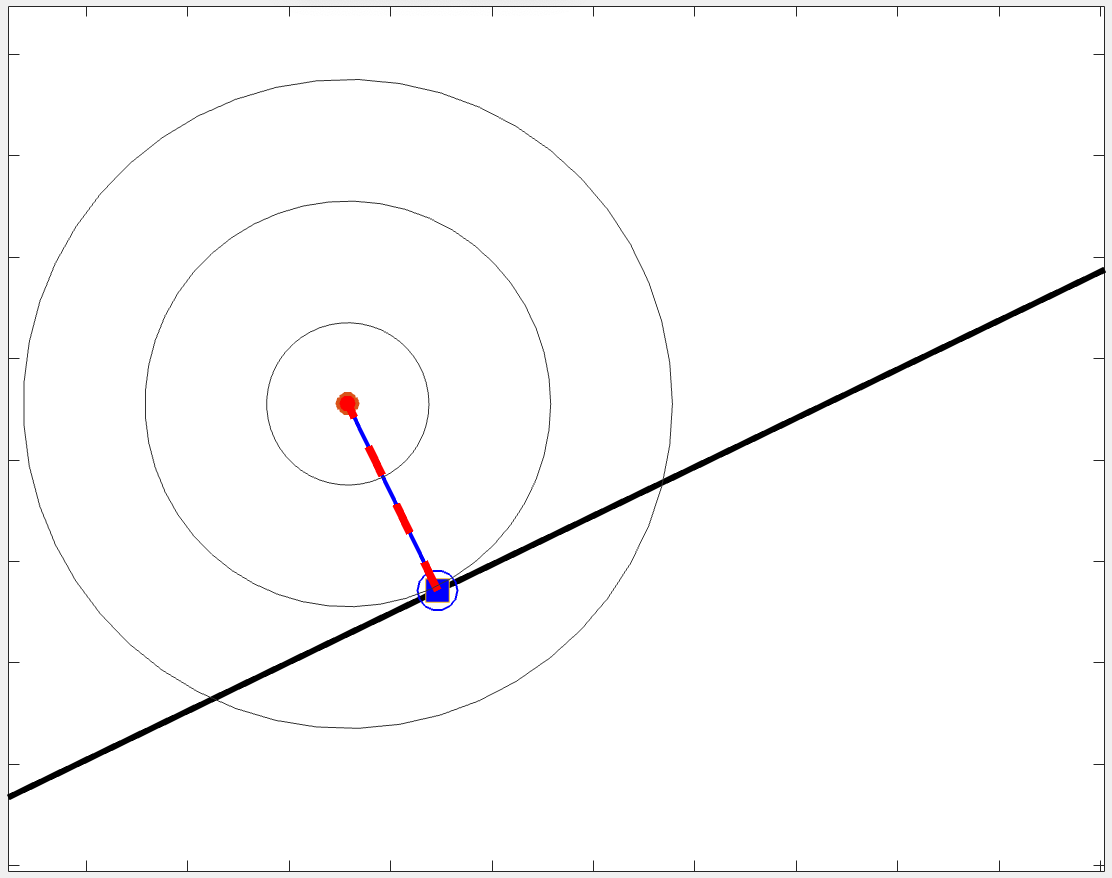
\includegraphics[width=0.7\linewidth]{fig1}
			\caption{An illustration of the problem}
		\end{figure}
		
		
		
	\end{flushleft}
\end{frame}







\myqrframe




\begin{frame}{Least squares with constraints}
	\begin{flushleft}
		
		\begin{small}
		\begin{equation}
			\begin{aligned}
				& \underset{\mathbf{x}}{\text{minimize}}
				& & \frac{1}{2} \bo{x}\T \bo{x}, \\
				& \text{subject to}
				& & \bo{A} \bo{x} = \bo{b}.
			\end{aligned}
		\end{equation}
		
		All solutions to $\bo{A} \bo{x} = \bo{b}$ are written as $\bo{x} = \bo{A}^+\bo{b} + \bo{N}\bo{z}$, where $\bo{N} = \text{null}(\bo{A})$, and $\bo{A}^+\bo{b} \in \text{row}(\bo{A})$ as we proved previously.  The cost function is:
		%
		\begin{align}
			f_c &= \frac{1}{2} (\bo{A}^+\bo{b} + \bo{N}\bo{z})\T (\bo{A}^+\bo{b} + \bo{N}\bo{z}) 
		\end{align}
		%
		We find extremum:
		%
		\begin{align}
			\frac{\partial f_c}{\partial \bo{z}} &= \bo{N}\T \bo{A}^+\bo{b} + \bo{N}\T\bo{N}\bo{z} = 0
			\\
			\bo{z} &= - \bo{N}\T \bo{A}^+\bo{b} 
			\\
			\bo{x} &= \bo{A}^+\bo{b} -  \bo{N}\bo{N}\T \bo{A}^+\bo{b} 
		\end{align}
		
		Columns of $\bo{A}^+$ lie in the row space of $\bo{A}$, so $\bo{N}\T \bo{A}^+ = 0$:
		%
		\begin{align}
			\bo{x} &= \bo{A}^+\bo{b}
		\end{align}
	\end{small}
		
	\end{flushleft}
\end{frame}


\end{document}
